% Options for packages loaded elsewhere
\PassOptionsToPackage{unicode}{hyperref}
\PassOptionsToPackage{hyphens}{url}
%
\documentclass[
]{article}
\usepackage{amsmath,amssymb}
\usepackage{iftex}
\ifPDFTeX
  \usepackage[T1]{fontenc}
  \usepackage[utf8]{inputenc}
  \usepackage{textcomp} % provide euro and other symbols
\else % if luatex or xetex
  \usepackage{unicode-math} % this also loads fontspec
  \defaultfontfeatures{Scale=MatchLowercase}
  \defaultfontfeatures[\rmfamily]{Ligatures=TeX,Scale=1}
\fi
\usepackage{lmodern}
\ifPDFTeX\else
  % xetex/luatex font selection
\fi
% Use upquote if available, for straight quotes in verbatim environments
\IfFileExists{upquote.sty}{\usepackage{upquote}}{}
\IfFileExists{microtype.sty}{% use microtype if available
  \usepackage[]{microtype}
  \UseMicrotypeSet[protrusion]{basicmath} % disable protrusion for tt fonts
}{}
\makeatletter
\@ifundefined{KOMAClassName}{% if non-KOMA class
  \IfFileExists{parskip.sty}{%
    \usepackage{parskip}
  }{% else
    \setlength{\parindent}{0pt}
    \setlength{\parskip}{6pt plus 2pt minus 1pt}}
}{% if KOMA class
  \KOMAoptions{parskip=half}}
\makeatother
\usepackage{xcolor}
\usepackage[margin=1in]{geometry}
\usepackage{color}
\usepackage{fancyvrb}
\newcommand{\VerbBar}{|}
\newcommand{\VERB}{\Verb[commandchars=\\\{\}]}
\DefineVerbatimEnvironment{Highlighting}{Verbatim}{commandchars=\\\{\}}
% Add ',fontsize=\small' for more characters per line
\usepackage{framed}
\definecolor{shadecolor}{RGB}{248,248,248}
\newenvironment{Shaded}{\begin{snugshade}}{\end{snugshade}}
\newcommand{\AlertTok}[1]{\textcolor[rgb]{0.94,0.16,0.16}{#1}}
\newcommand{\AnnotationTok}[1]{\textcolor[rgb]{0.56,0.35,0.01}{\textbf{\textit{#1}}}}
\newcommand{\AttributeTok}[1]{\textcolor[rgb]{0.13,0.29,0.53}{#1}}
\newcommand{\BaseNTok}[1]{\textcolor[rgb]{0.00,0.00,0.81}{#1}}
\newcommand{\BuiltInTok}[1]{#1}
\newcommand{\CharTok}[1]{\textcolor[rgb]{0.31,0.60,0.02}{#1}}
\newcommand{\CommentTok}[1]{\textcolor[rgb]{0.56,0.35,0.01}{\textit{#1}}}
\newcommand{\CommentVarTok}[1]{\textcolor[rgb]{0.56,0.35,0.01}{\textbf{\textit{#1}}}}
\newcommand{\ConstantTok}[1]{\textcolor[rgb]{0.56,0.35,0.01}{#1}}
\newcommand{\ControlFlowTok}[1]{\textcolor[rgb]{0.13,0.29,0.53}{\textbf{#1}}}
\newcommand{\DataTypeTok}[1]{\textcolor[rgb]{0.13,0.29,0.53}{#1}}
\newcommand{\DecValTok}[1]{\textcolor[rgb]{0.00,0.00,0.81}{#1}}
\newcommand{\DocumentationTok}[1]{\textcolor[rgb]{0.56,0.35,0.01}{\textbf{\textit{#1}}}}
\newcommand{\ErrorTok}[1]{\textcolor[rgb]{0.64,0.00,0.00}{\textbf{#1}}}
\newcommand{\ExtensionTok}[1]{#1}
\newcommand{\FloatTok}[1]{\textcolor[rgb]{0.00,0.00,0.81}{#1}}
\newcommand{\FunctionTok}[1]{\textcolor[rgb]{0.13,0.29,0.53}{\textbf{#1}}}
\newcommand{\ImportTok}[1]{#1}
\newcommand{\InformationTok}[1]{\textcolor[rgb]{0.56,0.35,0.01}{\textbf{\textit{#1}}}}
\newcommand{\KeywordTok}[1]{\textcolor[rgb]{0.13,0.29,0.53}{\textbf{#1}}}
\newcommand{\NormalTok}[1]{#1}
\newcommand{\OperatorTok}[1]{\textcolor[rgb]{0.81,0.36,0.00}{\textbf{#1}}}
\newcommand{\OtherTok}[1]{\textcolor[rgb]{0.56,0.35,0.01}{#1}}
\newcommand{\PreprocessorTok}[1]{\textcolor[rgb]{0.56,0.35,0.01}{\textit{#1}}}
\newcommand{\RegionMarkerTok}[1]{#1}
\newcommand{\SpecialCharTok}[1]{\textcolor[rgb]{0.81,0.36,0.00}{\textbf{#1}}}
\newcommand{\SpecialStringTok}[1]{\textcolor[rgb]{0.31,0.60,0.02}{#1}}
\newcommand{\StringTok}[1]{\textcolor[rgb]{0.31,0.60,0.02}{#1}}
\newcommand{\VariableTok}[1]{\textcolor[rgb]{0.00,0.00,0.00}{#1}}
\newcommand{\VerbatimStringTok}[1]{\textcolor[rgb]{0.31,0.60,0.02}{#1}}
\newcommand{\WarningTok}[1]{\textcolor[rgb]{0.56,0.35,0.01}{\textbf{\textit{#1}}}}
\usepackage{graphicx}
\makeatletter
\def\maxwidth{\ifdim\Gin@nat@width>\linewidth\linewidth\else\Gin@nat@width\fi}
\def\maxheight{\ifdim\Gin@nat@height>\textheight\textheight\else\Gin@nat@height\fi}
\makeatother
% Scale images if necessary, so that they will not overflow the page
% margins by default, and it is still possible to overwrite the defaults
% using explicit options in \includegraphics[width, height, ...]{}
\setkeys{Gin}{width=\maxwidth,height=\maxheight,keepaspectratio}
% Set default figure placement to htbp
\makeatletter
\def\fps@figure{htbp}
\makeatother
\setlength{\emergencystretch}{3em} % prevent overfull lines
\providecommand{\tightlist}{%
  \setlength{\itemsep}{0pt}\setlength{\parskip}{0pt}}
\setcounter{secnumdepth}{-\maxdimen} % remove section numbering
\ifLuaTeX
  \usepackage{selnolig}  % disable illegal ligatures
\fi
\usepackage{bookmark}
\IfFileExists{xurl.sty}{\usepackage{xurl}}{} % add URL line breaks if available
\urlstyle{same}
\hypersetup{
  pdftitle={PAC1},
  pdfauthor={Silvia Arroitajauregui Avilés},
  hidelinks,
  pdfcreator={LaTeX via pandoc}}

\title{PAC1}
\author{Silvia Arroitajauregui Avilés}
\date{2024-11-05}

\begin{document}
\maketitle

\section{Tabla de contenidos.}\label{tabla-de-contenidos.}

\section{Abstract.}\label{abstract.}

El presente trabajo tiene como objetivo realizar un acercamiento al
análisis de datos ómicos utilizando el dataset
\emph{2018-MetabotypingPaper}, así como RStudio y GitHub.

En primer lugar, se genera un repositorio en GitHub conectado al
proyecto en R y se crea el objeto \emph{SummarizedExperiment} a partir
del dataset.

Tras ello, se realiza una exploración del dataset que incluye
normalización, análisis de componentes principales, filtrado de
metabolitos y visualización de heatmaps.

Estos resultados parecen indicar patrones de correlación entre
metabolitos y factores individuales. No obstante, son necesarios más
estudios para poder concluir esto, pudiendo ser estos modelos
predictivos, análisis longitudinales y análisis de rutas metabólicas.

\section{Objetivos del estudio.}\label{objetivos-del-estudio.}

Los objetivos del presente trabajo son ejecutar un proceso simplificado
de análisis de datos ómicos, especificamente:

\begin{itemize}
\item
  Generar un proyecto en R y conectarlo a un repositorio en GitHub.
\item
  Crear un objeto Summarized Experiment a través del dataset escogido.
\item
  Realizar una exploración del dataset para tener una visión general de
  este.
\end{itemize}

\section{Materiales y métodos.}\label{materiales-y-muxe9todos.}

\subsection{Materiales utilizados.}\label{materiales-utilizados.}

Los materiales utilizados son el dataset \emph{2018-MetabotypingPaper}
(extraído del repositorio de GitHub metaboData, al cual puede accederse
a través de
\url{https://github.com/nutrimetabolomics/metaboData/tree/main/Datasets/2018-MetabotypingPaper}).

Este dataset fue utilizado en el paper ``\emph{Metabotypes of response
to bariatric surgery independent of the magnitude of weight loss}'' y
está conformado por:

\begin{itemize}
\item
  DataInfo\_S013.csv: Este archivo corresponde a los metadatos.
\item
  DataValues\_S013.csv: Valores clínicos y metabolómicos de 39 pacientes
  en 5 puntos temporales.
\item
  AAInformation\_S006.csv: Información adicional de los metabolitos de
  ``DataValues\_S013.csv''.
\end{itemize}

Así mismo, el estudio se realizará utilizando RStudio, con la versión de
R 4.4.1. Los paquetes utilizados se exploran en el apartado
\textbf{Métodos}.

Finalmente, para poder cargar todos nuestros documentos, será necesario
utilizar un repositorio de GitHub.

\subsection{Métodos.}\label{muxe9todos.}

\subsubsection{Creación del proyecto en R y del repositorio en
GitHub.}\label{creaciuxf3n-del-proyecto-en-r-y-del-repositorio-en-github.}

En primer lugar, crearemos el repositorio en GitHub. Para ello, con la
sesión iniciada, nos dirigiremos a \emph{Repositories / New}:

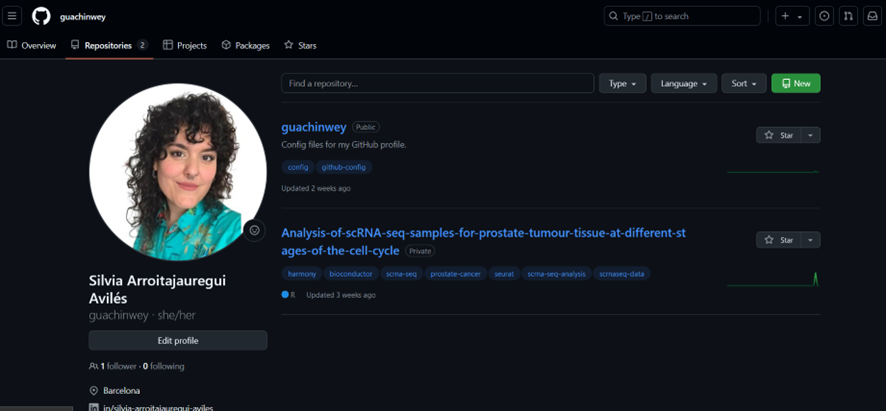
\includegraphics{images/clipboard-3636223962.png}

En la página de creación del Repositorio, tendremos que indicar el
nombre, una breve descripción y, en esta ocasión, lo haremos de dominio
público. Tras ello, clicaremos en \emph{Create repository:}

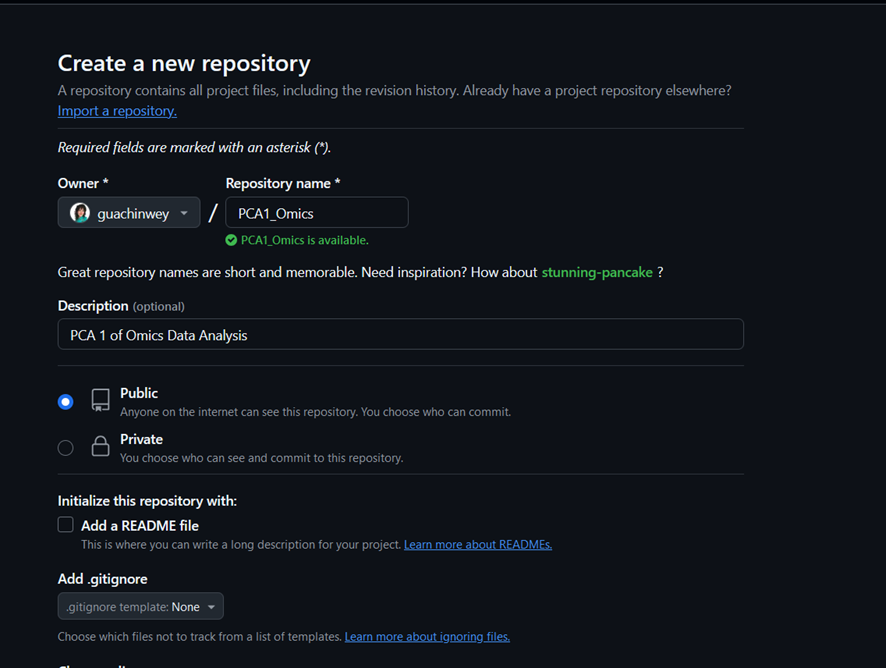
\includegraphics{images/clipboard-3557996507.png}

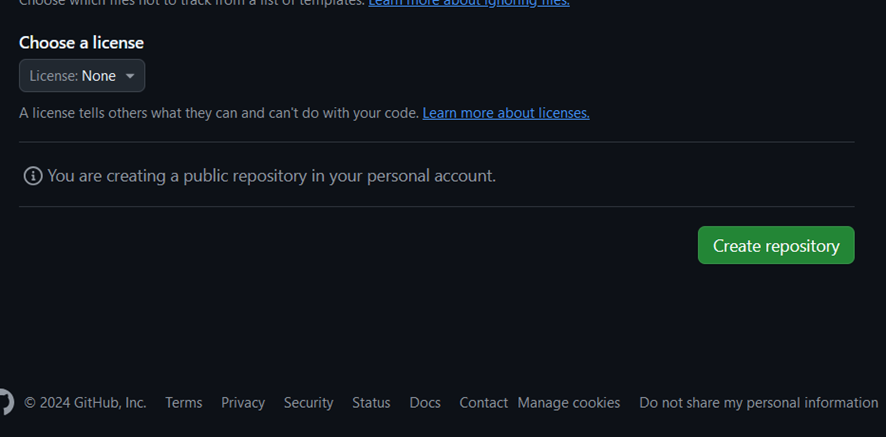
\includegraphics{images/clipboard-2127165342.png}

Esto nos creará el repositorio, el enlace del cual deberemos copiar en
RStudio:

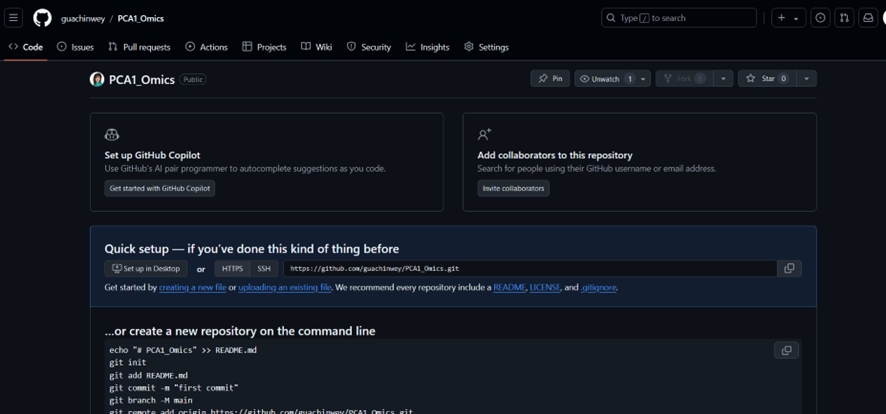
\includegraphics{images/clipboard-3940631010.png}

En RStudio, nos dirigimos a \emph{File / New Project / Version Control /
Git}. En la pantalla final, deberemos copiar la URL del repositorio
creado, así como indicar la dirección local del proyecto en nuestro
ordenador:

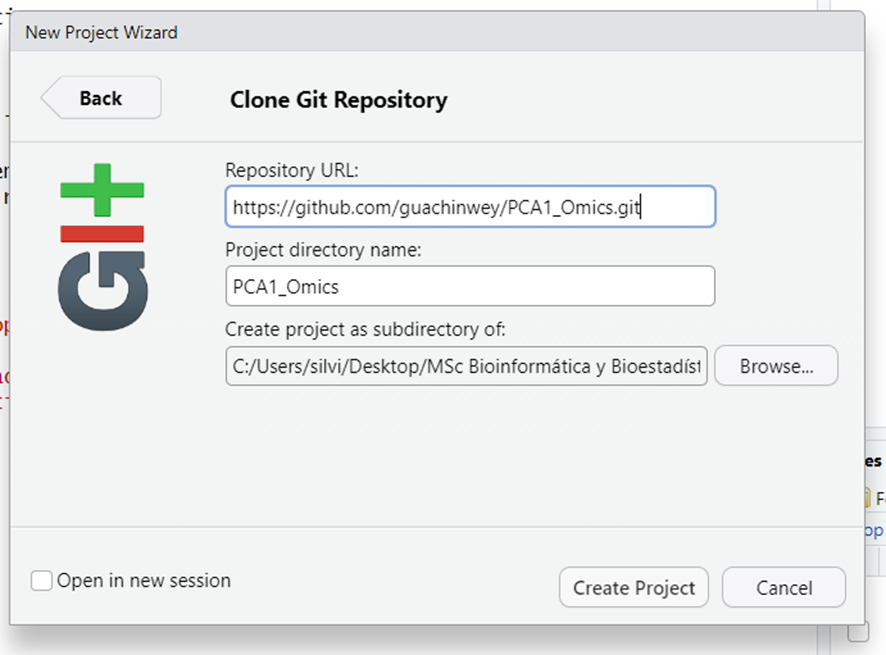
\includegraphics{images/clipboard-4094692892.png}

Finalmente, para sincronizar RStudio con GitHub, deberemos ir haciendo
\emph{Commit} en las actualizaciones que generemos:

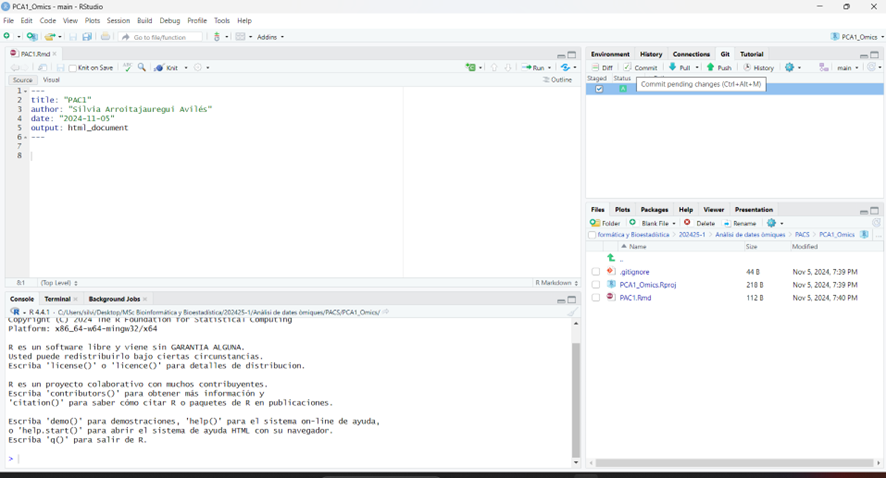
\includegraphics{images/clipboard-30791053.png}

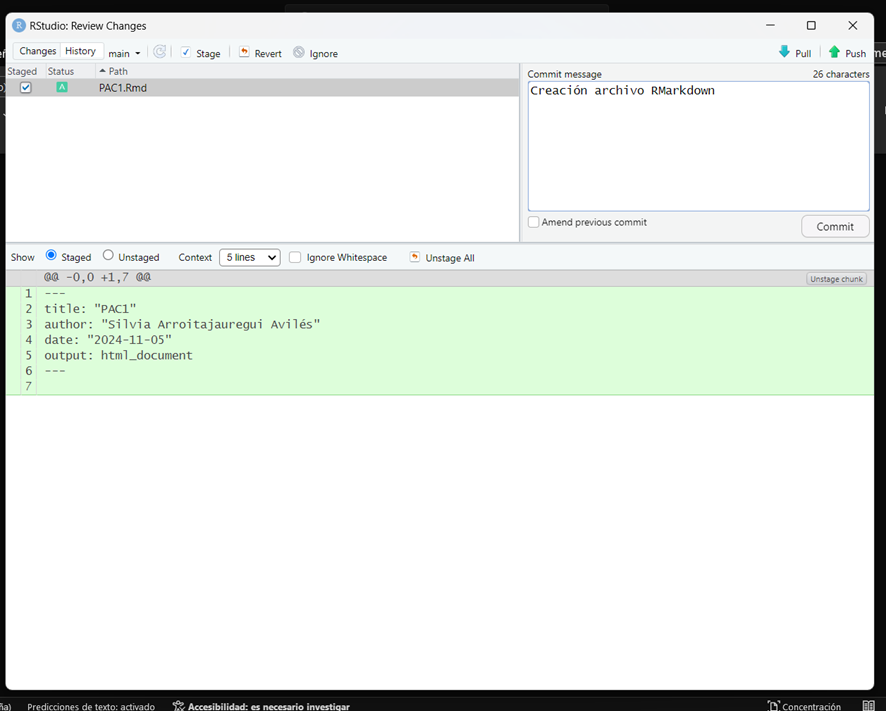
\includegraphics{images/clipboard-2508258357.png}

Y con un simple click en \emph{Push} estos quedarán actualizados en
GitHub:

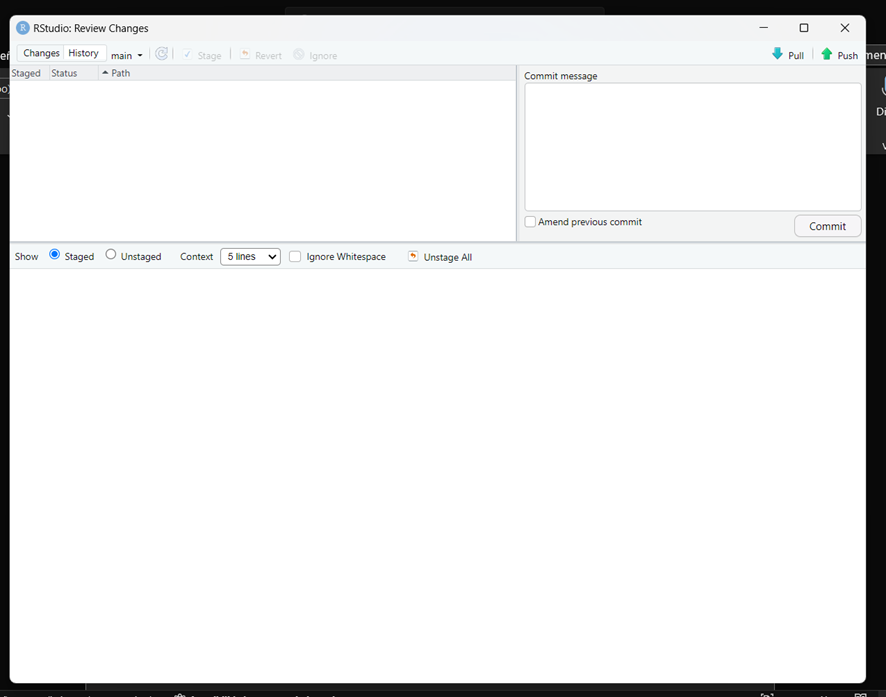
\includegraphics{images/clipboard-2370911352.png}

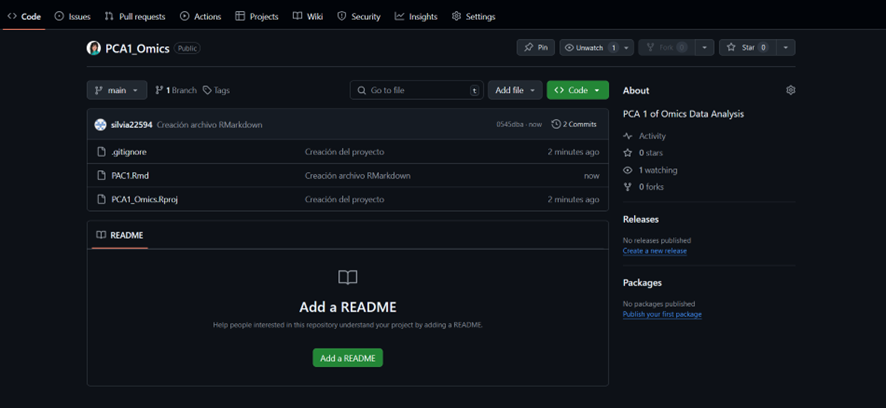
\includegraphics{images/clipboard-2395957737.png}

\subsection{Análisis en R.}\label{anuxe1lisis-en-r.}

Para generar el objeto \emph{Summarized experiment} y realizar su
posterior análisis, se utilizarán una serie de repositorios y librerias
de R, a destacar el repositorio \emph{Bioconductor} y su libreria
\emph{Summarized Experiment}, además de otras que se verán en el
apartado \textbf{Resultados}.

Tras obtener el objeto, se hará un primer análisis exploratorio de
datos, continuando por normalizar el dataset, así como realizar el
cálculo de PCA. También se harán estudios de la distribución de las
variables y heatmaps para revisar la relación entre los metabolitos,
estos últimos con los datos originales y con un posterior filtrado.

\section{Resultados.}\label{resultados.}

\subsection{Descarga de datos.}\label{descarga-de-datos.}

Para la descarga de datos escogeremos los archivos DataValues\_S013.csv
y DataInfo\_S013.csv:

\begin{Shaded}
\begin{Highlighting}[]
\CommentTok{\# Indicamos los enlaces de descarga del dataset:}
\NormalTok{link\_DataValues }\OtherTok{\textless{}{-}} \StringTok{"https://raw.githubusercontent.com/nutrimetabolomics/metaboData/main/Datasets/2018{-}MetabotypingPaper/DataValues\_S013.csv"}
\NormalTok{link\_DataInfo }\OtherTok{\textless{}{-}} \StringTok{"https://raw.githubusercontent.com/nutrimetabolomics/metaboData/main/Datasets/2018{-}MetabotypingPaper/DataInfo\_S013.csv"}
\end{Highlighting}
\end{Shaded}

\begin{Shaded}
\begin{Highlighting}[]
\CommentTok{\# Ponemos nombre a los archivos:}
\NormalTok{DataValues }\OtherTok{\textless{}{-}} \StringTok{"DataValues\_S013.csv"}
\NormalTok{DataInfo }\OtherTok{\textless{}{-}} \StringTok{"DataInfo\_S013.csv"}
\end{Highlighting}
\end{Shaded}

\begin{Shaded}
\begin{Highlighting}[]
\CommentTok{\# Procedemos a la descarga:}
\FunctionTok{download.file}\NormalTok{(link\_DataValues, }\AttributeTok{destfile =}\NormalTok{ DataValues)}
\FunctionTok{download.file}\NormalTok{(link\_DataInfo, }\AttributeTok{destfile =}\NormalTok{ DataInfo)}
\end{Highlighting}
\end{Shaded}

\begin{Shaded}
\begin{Highlighting}[]
\CommentTok{\# Finalmente, cargamos nuestros archivos:}
\NormalTok{data\_values }\OtherTok{\textless{}{-}} \FunctionTok{read.csv}\NormalTok{(DataValues, }\AttributeTok{row.names =} \DecValTok{1}\NormalTok{)}
\NormalTok{data\_info }\OtherTok{\textless{}{-}} \FunctionTok{read.csv}\NormalTok{(DataInfo, }\AttributeTok{row.names =} \DecValTok{1}\NormalTok{)}
\end{Highlighting}
\end{Shaded}

\subsection{\texorpdfstring{Creación del objeto \emph{Summarized
Experiment}.}{Creación del objeto Summarized Experiment.}}\label{creaciuxf3n-del-objeto-summarized-experiment.}

Tras revisar los archivos, vemos que en primer lugar debemos transponer
data\_values, ya que es importante que en el \emph{assay} tengamos las
muestras en columnas y los metabólitos en filas:

\begin{Shaded}
\begin{Highlighting}[]
\NormalTok{data\_values }\OtherTok{\textless{}{-}} \FunctionTok{t}\NormalTok{(data\_values)}
\end{Highlighting}
\end{Shaded}

Además, observamos, gracias a data\_info, que los metadatos son las
primeras nueve columnas de data\_values (\emph{Subjects, Surgery, Age,
Gender, Group}, y 4 mediciones de metabólitos iniciales que tienen
valores categóricos). Vamos a separarlos para que se identifiquen como
metadatos:

\begin{Shaded}
\begin{Highlighting}[]
\NormalTok{metadata }\OtherTok{\textless{}{-}}\NormalTok{ data\_values[}\DecValTok{1}\SpecialCharTok{:}\DecValTok{9}\NormalTok{,]}
\NormalTok{metadata }\OtherTok{\textless{}{-}} \FunctionTok{t}\NormalTok{(metadata)}
\NormalTok{metadata }\OtherTok{\textless{}{-}} \FunctionTok{as.data.frame}\NormalTok{(metadata)}
\NormalTok{assay\_data }\OtherTok{\textless{}{-}}\NormalTok{ data\_values[}\SpecialCharTok{{-}}\FunctionTok{c}\NormalTok{(}\DecValTok{1}\SpecialCharTok{:}\DecValTok{9}\NormalTok{), ]}
\end{Highlighting}
\end{Shaded}

Ponemos los sujetos como identificativo de fila en metadata y de las
columnas de assay\_data:

\begin{Shaded}
\begin{Highlighting}[]
\FunctionTok{rownames}\NormalTok{(metadata) }\OtherTok{\textless{}{-}}\NormalTok{ metadata}\SpecialCharTok{$}\NormalTok{SUBJECTS}
\FunctionTok{colnames}\NormalTok{(assay\_data) }\OtherTok{\textless{}{-}}\NormalTok{ metadata}\SpecialCharTok{$}\NormalTok{SUBJECTS}
\end{Highlighting}
\end{Shaded}

Convertimos a numéricas las columnas de metadatos correspondientes para
facilitar el posterior análisis:

\begin{Shaded}
\begin{Highlighting}[]
\NormalTok{metadata}\SpecialCharTok{$}\NormalTok{SUBJECTS }\OtherTok{\textless{}{-}} \FunctionTok{as.numeric}\NormalTok{(metadata}\SpecialCharTok{$}\NormalTok{SUBJECTS)}
\NormalTok{metadata}\SpecialCharTok{$}\NormalTok{AGE }\OtherTok{\textless{}{-}} \FunctionTok{as.numeric}\NormalTok{(metadata}\SpecialCharTok{$}\NormalTok{AGE)}
\NormalTok{metadata}\SpecialCharTok{$}\NormalTok{MEDDM\_T0 }\OtherTok{\textless{}{-}} \FunctionTok{as.numeric}\NormalTok{(metadata}\SpecialCharTok{$}\NormalTok{MEDDM\_T0)}
\NormalTok{metadata}\SpecialCharTok{$}\NormalTok{MEDCOL\_T0 }\OtherTok{\textless{}{-}} \FunctionTok{as.numeric}\NormalTok{(metadata}\SpecialCharTok{$}\NormalTok{MEDCOL\_T0)}
\NormalTok{metadata}\SpecialCharTok{$}\NormalTok{MEDINF\_T0 }\OtherTok{\textless{}{-}} \FunctionTok{as.numeric}\NormalTok{(metadata}\SpecialCharTok{$}\NormalTok{MEDINF\_T0)}
\NormalTok{metadata}\SpecialCharTok{$}\NormalTok{MEDHTA\_T0 }\OtherTok{\textless{}{-}} \FunctionTok{as.numeric}\NormalTok{(metadata}\SpecialCharTok{$}\NormalTok{MEDHTA\_T0)}
\FunctionTok{str}\NormalTok{(metadata)}
\end{Highlighting}
\end{Shaded}

\begin{verbatim}
## 'data.frame':    39 obs. of  9 variables:
##  $ SUBJECTS : num  1 2 3 4 5 6 7 8 9 10 ...
##  $ SURGERY  : chr  "by pass" "by pass" "by pass" "by pass" ...
##  $ AGE      : num  27 19 42 37 42 24 33 55 40 47 ...
##  $ GENDER   : chr  "F" "F" "F" "F" ...
##  $ Group    : chr  "1" "2" "1" "2" ...
##  $ MEDDM_T0 : num  0 0 0 0 0 0 0 0 0 0 ...
##  $ MEDCOL_T0: num  0 0 0 0 0 0 0 0 0 0 ...
##  $ MEDINF_T0: num  0 0 0 0 0 0 0 1 0 0 ...
##  $ MEDHTA_T0: num  1 0 0 0 0 0 0 0 0 0 ...
\end{verbatim}

Forzamos los metadatos a ser reconocidos como tal:

\begin{Shaded}
\begin{Highlighting}[]
\FunctionTok{library}\NormalTok{(S4Vectors)}
\end{Highlighting}
\end{Shaded}

\begin{verbatim}
## Cargando paquete requerido: stats4
\end{verbatim}

\begin{verbatim}
## Cargando paquete requerido: BiocGenerics
\end{verbatim}

\begin{verbatim}
## 
## Adjuntando el paquete: 'BiocGenerics'
\end{verbatim}

\begin{verbatim}
## The following objects are masked from 'package:stats':
## 
##     IQR, mad, sd, var, xtabs
\end{verbatim}

\begin{verbatim}
## The following objects are masked from 'package:base':
## 
##     anyDuplicated, aperm, append, as.data.frame, basename, cbind,
##     colnames, dirname, do.call, duplicated, eval, evalq, Filter, Find,
##     get, grep, grepl, intersect, is.unsorted, lapply, Map, mapply,
##     match, mget, order, paste, pmax, pmax.int, pmin, pmin.int,
##     Position, rank, rbind, Reduce, rownames, sapply, saveRDS, setdiff,
##     table, tapply, union, unique, unsplit, which.max, which.min
\end{verbatim}

\begin{verbatim}
## 
## Adjuntando el paquete: 'S4Vectors'
\end{verbatim}

\begin{verbatim}
## The following object is masked from 'package:utils':
## 
##     findMatches
\end{verbatim}

\begin{verbatim}
## The following objects are masked from 'package:base':
## 
##     expand.grid, I, unname
\end{verbatim}

\begin{Shaded}
\begin{Highlighting}[]
\NormalTok{colData }\OtherTok{\textless{}{-}} \FunctionTok{DataFrame}\NormalTok{(}\AttributeTok{Subjects =}\NormalTok{ metadata}\SpecialCharTok{$}\NormalTok{SUBJECTS,}
                     \AttributeTok{Surgery =}\NormalTok{ metadata}\SpecialCharTok{$}\NormalTok{SURGERY,}
                     \AttributeTok{Age =}\NormalTok{ metadata}\SpecialCharTok{$}\NormalTok{AGE, }
                     \AttributeTok{Gender =}\NormalTok{ metadata}\SpecialCharTok{$}\NormalTok{GENDER,}
                     \AttributeTok{Group =}\NormalTok{ metadata}\SpecialCharTok{$}\NormalTok{Group,}
                     \AttributeTok{MEDMM\_T0 =}\NormalTok{ metadata}\SpecialCharTok{$}\NormalTok{MEDDM\_T0, }
                     \AttributeTok{MEDCOL\_T0 =}\NormalTok{ metadata}\SpecialCharTok{$}\NormalTok{MEDCOL\_T0, }
                     \AttributeTok{MEDINF\_T0 =}\NormalTok{ metadata}\SpecialCharTok{$}\NormalTok{MEDINF\_T0, }
                     \AttributeTok{MEDHTA\_T0 =}\NormalTok{ metadata}\SpecialCharTok{$}\NormalTok{MEDHTA\_T0)}
\end{Highlighting}
\end{Shaded}

En \emph{assay\_data}, detectamos que se están almacenando los datos
como carácteres, convertimos también a numéricos y transformamos los NA
por 0:

\begin{Shaded}
\begin{Highlighting}[]
\CommentTok{\# Convertimos los NA a 0:}
\NormalTok{assay\_data[}\FunctionTok{is.na}\NormalTok{(assay\_data)] }\OtherTok{\textless{}{-}} \DecValTok{0} 

\CommentTok{\# Transformamos assay\_data en una matriz de 39 columnas y 686 filas:}
\NormalTok{assay\_data }\OtherTok{\textless{}{-}} \FunctionTok{as.matrix}\NormalTok{ (assay\_data)}
\NormalTok{assay\_data }\OtherTok{\textless{}{-}} \FunctionTok{matrix}\NormalTok{(}\FunctionTok{as.numeric}\NormalTok{(assay\_data), }\AttributeTok{nrow =} \DecValTok{686}\NormalTok{, }\AttributeTok{ncol =} \DecValTok{39}\NormalTok{)}

\CommentTok{\# Indicamos que los identificativos de las filas serán los metabólitos y los de las columnas los sujetos:}
\FunctionTok{rownames}\NormalTok{(assay\_data) }\OtherTok{\textless{}{-}} \FunctionTok{rownames}\NormalTok{(data\_values)[}\SpecialCharTok{{-}}\FunctionTok{c}\NormalTok{(}\DecValTok{1}\SpecialCharTok{:}\DecValTok{9}\NormalTok{)]}
\FunctionTok{colnames}\NormalTok{(assay\_data) }\OtherTok{\textless{}{-}}\NormalTok{ metadata}\SpecialCharTok{$}\NormalTok{SUBJECTS}
\end{Highlighting}
\end{Shaded}

Hacemos un análisis inicial para comprobar que la generación del objeto
\emph{summarized\_object} será correcta. Para ello, comprobamos que las
dimensiones de \emph{assay\_data} y \emph{colDat}a son compatibles.

También comprobamos que los nombres de las filas de \emph{colData} sean
los mismos que los nombres de las columnas de \emph{assay\_data}, lo que
servirá para identificar de cada muestra sus metadatos.

\begin{Shaded}
\begin{Highlighting}[]
\FunctionTok{print}\NormalTok{(}\FunctionTok{dim}\NormalTok{(assay\_data))}
\end{Highlighting}
\end{Shaded}

\begin{verbatim}
## [1] 686  39
\end{verbatim}

\begin{Shaded}
\begin{Highlighting}[]
\FunctionTok{print}\NormalTok{(}\FunctionTok{dim}\NormalTok{(colData))}
\end{Highlighting}
\end{Shaded}

\begin{verbatim}
## [1] 39  9
\end{verbatim}

\begin{Shaded}
\begin{Highlighting}[]
\FunctionTok{print}\NormalTok{(}\FunctionTok{all}\NormalTok{(}\FunctionTok{rownames}\NormalTok{(colData) }\SpecialCharTok{==} \FunctionTok{colnames}\NormalTok{(assay\_data)))}
\end{Highlighting}
\end{Shaded}

\begin{verbatim}
## [1] TRUE
\end{verbatim}

Ahora tenemos que cargar la libreria \emph{SummarizedExperiment} para
poder generar el objeto homónimo:

\begin{Shaded}
\begin{Highlighting}[]
\FunctionTok{library}\NormalTok{(SummarizedExperiment)}
\end{Highlighting}
\end{Shaded}

\begin{verbatim}
## Cargando paquete requerido: MatrixGenerics
\end{verbatim}

\begin{verbatim}
## Cargando paquete requerido: matrixStats
\end{verbatim}

\begin{verbatim}
## 
## Adjuntando el paquete: 'MatrixGenerics'
\end{verbatim}

\begin{verbatim}
## The following objects are masked from 'package:matrixStats':
## 
##     colAlls, colAnyNAs, colAnys, colAvgsPerRowSet, colCollapse,
##     colCounts, colCummaxs, colCummins, colCumprods, colCumsums,
##     colDiffs, colIQRDiffs, colIQRs, colLogSumExps, colMadDiffs,
##     colMads, colMaxs, colMeans2, colMedians, colMins, colOrderStats,
##     colProds, colQuantiles, colRanges, colRanks, colSdDiffs, colSds,
##     colSums2, colTabulates, colVarDiffs, colVars, colWeightedMads,
##     colWeightedMeans, colWeightedMedians, colWeightedSds,
##     colWeightedVars, rowAlls, rowAnyNAs, rowAnys, rowAvgsPerColSet,
##     rowCollapse, rowCounts, rowCummaxs, rowCummins, rowCumprods,
##     rowCumsums, rowDiffs, rowIQRDiffs, rowIQRs, rowLogSumExps,
##     rowMadDiffs, rowMads, rowMaxs, rowMeans2, rowMedians, rowMins,
##     rowOrderStats, rowProds, rowQuantiles, rowRanges, rowRanks,
##     rowSdDiffs, rowSds, rowSums2, rowTabulates, rowVarDiffs, rowVars,
##     rowWeightedMads, rowWeightedMeans, rowWeightedMedians,
##     rowWeightedSds, rowWeightedVars
\end{verbatim}

\begin{verbatim}
## Cargando paquete requerido: GenomicRanges
\end{verbatim}

\begin{verbatim}
## Cargando paquete requerido: IRanges
\end{verbatim}

\begin{verbatim}
## 
## Adjuntando el paquete: 'IRanges'
\end{verbatim}

\begin{verbatim}
## The following object is masked from 'package:grDevices':
## 
##     windows
\end{verbatim}

\begin{verbatim}
## Cargando paquete requerido: GenomeInfoDb
\end{verbatim}

\begin{verbatim}
## Cargando paquete requerido: Biobase
\end{verbatim}

\begin{verbatim}
## Welcome to Bioconductor
## 
##     Vignettes contain introductory material; view with
##     'browseVignettes()'. To cite Bioconductor, see
##     'citation("Biobase")', and for packages 'citation("pkgname")'.
\end{verbatim}

\begin{verbatim}
## 
## Adjuntando el paquete: 'Biobase'
\end{verbatim}

\begin{verbatim}
## The following object is masked from 'package:MatrixGenerics':
## 
##     rowMedians
\end{verbatim}

\begin{verbatim}
## The following objects are masked from 'package:matrixStats':
## 
##     anyMissing, rowMedians
\end{verbatim}

Creamos el objeto SummarizedExperiment. Para ello, usaremos
\emph{assay\_data} como datos y \emph{colData} como metadatos:

\begin{Shaded}
\begin{Highlighting}[]
\NormalTok{summarized\_experiment }\OtherTok{\textless{}{-}} \FunctionTok{SummarizedExperiment}\NormalTok{(}\AttributeTok{assays =} \FunctionTok{list}\NormalTok{(}\AttributeTok{counts =}\NormalTok{ assay\_data), }\AttributeTok{colData =}\NormalTok{ colData)}
\end{Highlighting}
\end{Shaded}

\subsection{\texorpdfstring{Guardado del objeto \emph{Summarized
experiment.}}{Guardado del objeto Summarized experiment.}}\label{guardado-del-objeto-summarized-experiment.}

Guardamos el objeto summarized\_experiment como archivo .RDA:

\begin{Shaded}
\begin{Highlighting}[]
\FunctionTok{save}\NormalTok{(summarized\_experiment, }\AttributeTok{file =} \StringTok{"summarized\_experiment.RDA"}\NormalTok{)}
\end{Highlighting}
\end{Shaded}

\subsection{Análisis del dataset.}\label{anuxe1lisis-del-dataset.}

En primer lugar, revisamos el objeto \emph{summarized\_experiment}. Con
esto, podemos confirmar las dimensiones (686 metabolitos y 39 muestras),
que solo tiene un assay, en formato de concentración de metabolitos y
que tiene metadatos en \emph{colData} sobre cada muestra, formado por 9
variables.

\begin{Shaded}
\begin{Highlighting}[]
\NormalTok{summarized\_experiment}
\end{Highlighting}
\end{Shaded}

\begin{verbatim}
## class: SummarizedExperiment 
## dim: 686 39 
## metadata(0):
## assays(1): counts
## rownames(686): GLU_T0 INS_T0 ... SM.C24.0_T5 SM.C24.1_T5
## rowData names(0):
## colnames(39): 1 2 ... 38 39
## colData names(9): Subjects Surgery ... MEDINF_T0 MEDHTA_T0
\end{verbatim}

Si revisamos los metadatos de \emph{colData}, podemos confirmar las 9
variables por muestra:

\begin{Shaded}
\begin{Highlighting}[]
\FunctionTok{colData}\NormalTok{(summarized\_experiment)}
\end{Highlighting}
\end{Shaded}

\begin{verbatim}
## DataFrame with 39 rows and 9 columns
##      Subjects     Surgery       Age      Gender       Group  MEDMM_T0 MEDCOL_T0
##     <numeric> <character> <numeric> <character> <character> <numeric> <numeric>
## 1           1     by pass        27           F           1         0         0
## 2           2     by pass        19           F           2         0         0
## 3           3     by pass        42           F           1         0         0
## 4           4     by pass        37           F           2         0         0
## 5           5     tubular        42           F           1         0         0
## ...       ...         ...       ...         ...         ...       ...       ...
## 35         35     tubular        39           M           2         0         0
## 36         36     tubular        35           M           1         0         0
## 37         37     by pass        46           M           2         0         0
## 38         38     tubular        41           M           1         0         0
## 39         39     by pass        26           M           1         0         0
##     MEDINF_T0 MEDHTA_T0
##     <numeric> <numeric>
## 1           0         1
## 2           0         0
## 3           0         0
## 4           0         0
## 5           0         0
## ...       ...       ...
## 35          0         1
## 36          0         0
## 37          1         0
## 38          0         0
## 39          0         0
\end{verbatim}

Revisando las filas de \emph{assay}, obtenemos un listado de los
metabolitos:

\begin{Shaded}
\begin{Highlighting}[]
\FunctionTok{head}\NormalTok{(}\FunctionTok{rownames}\NormalTok{(}\FunctionTok{assay}\NormalTok{(summarized\_experiment)))}
\end{Highlighting}
\end{Shaded}

\begin{verbatim}
## [1] "GLU_T0"            "INS_T0"            "HOMA_T0"          
## [4] "HBA1C_T0"          "HBA1C.mmol.mol_T0" "PESO_T0"
\end{verbatim}

\subsection{Resumen inicial del
dataset.}\label{resumen-inicial-del-dataset.}

Hacemos un primer resumen de los datos:

\begin{Shaded}
\begin{Highlighting}[]
\FunctionTok{summary}\NormalTok{(}\FunctionTok{assay}\NormalTok{(summarized\_experiment))}
\end{Highlighting}
\end{Shaded}

\begin{verbatim}
##        1                  2                3                 4         
##  Min.   :-99.0000   Min.   : -9.00   Min.   :-99.000   Min.   :-99.00  
##  1st Qu.:  0.4425   1st Qu.:  0.00   1st Qu.:  0.540   1st Qu.:  0.52  
##  Median :  3.3000   Median :  1.32   Median :  3.735   Median :  4.49  
##  Mean   : 36.7822   Mean   : 32.76   Mean   : 34.580   Mean   : 41.23  
##  3rd Qu.: 33.0000   3rd Qu.: 24.93   3rd Qu.: 33.830   3rd Qu.: 41.60  
##  Max.   :876.0000   Max.   :951.00   Max.   :723.000   Max.   :987.00  
##        5                   6                   7                 8           
##  Min.   : -99.0000   Min.   : -99.0000   Min.   :  -9.00   Min.   :-99.0000  
##  1st Qu.:   0.3892   1st Qu.:   0.5525   1st Qu.:   0.00   1st Qu.:  0.4925  
##  Median :   2.7150   Median :   3.9950   Median :   1.23   Median :  4.0700  
##  Mean   :  38.7642   Mean   :  42.8119   Mean   :  31.10   Mean   : 39.3962  
##  3rd Qu.:  41.1750   3rd Qu.:  38.4500   3rd Qu.:  18.70   3rd Qu.: 43.4500  
##  Max.   :1070.0000   Max.   :1320.0000   Max.   :1250.00   Max.   :926.0000  
##        9                 10               11                12         
##  Min.   : -99.00   Min.   :-99.00   Min.   :-99.000   Min.   :-99.000  
##  1st Qu.:   0.00   1st Qu.:  0.00   1st Qu.:  0.000   1st Qu.:  0.920  
##  Median :   1.16   Median :  1.03   Median :  0.885   Median :  4.115  
##  Mean   :  32.96   Mean   : 32.74   Mean   : 30.104   Mean   : 40.668  
##  3rd Qu.:  21.43   3rd Qu.: 24.75   3rd Qu.: 18.650   3rd Qu.: 39.475  
##  Max.   :1150.00   Max.   :954.00   Max.   :892.000   Max.   :746.000  
##        13                 14                15                 16          
##  Min.   :-99.0000   Min.   : -99.00   Min.   :  -9.000   Min.   : -9.0000  
##  1st Qu.:  0.8608   1st Qu.:   0.59   1st Qu.:   0.570   1st Qu.:  0.5225  
##  Median :  4.1100   Median :   4.14   Median :   4.805   Median :  3.9400  
##  Mean   : 38.6822   Mean   :  46.03   Mean   :  50.166   Mean   : 42.5622  
##  3rd Qu.: 41.0000   3rd Qu.:  41.60   3rd Qu.:  56.025   3rd Qu.: 43.0500  
##  Max.   :654.0000   Max.   :1050.00   Max.   :1350.000   Max.   :833.0000  
##        17                18                 19                 20           
##  Min.   : -99.00   Min.   :  -9.000   Min.   : -9.0000   Min.   : -99.0000  
##  1st Qu.:   0.53   1st Qu.:   0.500   1st Qu.:  0.5308   1st Qu.:   0.5748  
##  Median :   4.49   Median :   4.145   Median :  4.1900   Median :   5.0350  
##  Mean   :  45.91   Mean   :  49.194   Mean   : 42.2168   Mean   :  45.2580  
##  3rd Qu.:  43.67   3rd Qu.:  47.450   3rd Qu.: 39.9000   3rd Qu.:  46.9750  
##  Max.   :1040.00   Max.   :1560.000   Max.   :863.0000   Max.   :1240.0000  
##        21                 22                23                24          
##  Min.   : -9.0000   Min.   : -99.00   Min.   :-99.000   Min.   : -99.000  
##  1st Qu.:  0.4625   1st Qu.:   0.00   1st Qu.:  0.350   1st Qu.:   0.645  
##  Median :  3.2500   Median :   0.98   Median :  2.665   Median :   4.820  
##  Mean   : 35.3213   Mean   :  36.12   Mean   : 35.076   Mean   :  51.008  
##  3rd Qu.: 34.9750   3rd Qu.:  21.60   3rd Qu.: 32.000   3rd Qu.:  49.525  
##  Max.   :677.0000   Max.   :1230.00   Max.   :965.000   Max.   :1280.000  
##        25                 26                 27                28         
##  Min.   :-99.0000   Min.   :-99.0000   Min.   :-99.000   Min.   :-99.000  
##  1st Qu.:  0.4725   1st Qu.:  0.4325   1st Qu.:  0.450   1st Qu.:  0.000  
##  Median :  3.4300   Median :  3.4200   Median :  3.155   Median :  0.018  
##  Mean   : 41.3190   Mean   : 33.7009   Mean   : 39.297   Mean   : 20.098  
##  3rd Qu.: 43.0000   3rd Qu.: 32.9000   3rd Qu.: 38.975   3rd Qu.:  4.662  
##  Max.   :935.0000   Max.   :871.0000   Max.   :907.000   Max.   :713.000  
##        29               30                 31                32         
##  Min.   :-99.00   Min.   : -99.000   Min.   : -99.00   Min.   : -9.000  
##  1st Qu.:  0.00   1st Qu.:   0.720   1st Qu.:   0.00   1st Qu.:  0.380  
##  Median :  1.23   Median :   5.615   Median :   1.24   Median :  2.735  
##  Mean   : 31.51   Mean   :  56.929   Mean   :  39.08   Mean   : 38.141  
##  3rd Qu.: 24.45   3rd Qu.:  58.750   3rd Qu.:  23.93   3rd Qu.: 35.975  
##  Max.   :846.00   Max.   :1240.000   Max.   :1140.00   Max.   :921.000  
##        33                34                  35                 36         
##  Min.   : -9.000   Min.   : -99.0000   Min.   : -9.0000   Min.   : -9.000  
##  1st Qu.:  0.390   1st Qu.:   0.0512   1st Qu.:  0.3925   1st Qu.:  0.000  
##  Median :  2.425   Median :   1.5050   Median :  3.1000   Median :  0.000  
##  Mean   : 36.208   Mean   :  36.9961   Mean   : 41.1227   Mean   : 20.247  
##  3rd Qu.: 36.475   3rd Qu.:  23.6250   3rd Qu.: 38.5850   3rd Qu.:  4.562  
##  Max.   :903.000   Max.   :1220.0000   Max.   :990.0000   Max.   :562.000  
##        37                38               39         
##  Min.   :-99.000   Min.   : -9.00   Min.   :-99.000  
##  1st Qu.:  0.000   1st Qu.:  0.00   1st Qu.:  0.000  
##  Median :  0.000   Median :  0.76   Median :  0.057  
##  Mean   : 18.263   Mean   : 26.98   Mean   : 23.597  
##  3rd Qu.:  4.157   3rd Qu.: 16.45   3rd Qu.:  5.085  
##  Max.   :593.000   Max.   :680.00   Max.   :552.000
\end{verbatim}

Vamos a reforzar estos resultados con un boxplot para poder revisar
mejor los estadísticos:

\begin{Shaded}
\begin{Highlighting}[]
\FunctionTok{boxplot}\NormalTok{(}\FunctionTok{assay}\NormalTok{(summarized\_experiment))}
\end{Highlighting}
\end{Shaded}

\includegraphics{Informe_files/figure-latex/unnamed-chunk-19-1.pdf}

Con estos resultados, podemos observar lo siguiente:

\begin{itemize}
\item
  Vemos puntos mínimos en negativo, como -99 (muestras 1, 4, 5\ldots) y
  -9, pudiendo ser valores faltantes o errores en la medición, dando
  lugar a datos inválidos.
\item
  Se observan valores máximos muy altos (1560 en la muestra 18) en
  comparación con el resto, por lo que sería interesante estudiar la
  presencia de outliers que pudieran afectar el análisis.
\item
  Vemos las medianas y los valores medios bastante distintos, por lo que
  los datos podrían ser asimétricos.
\item
  El rango de los datos es muy amplio, como se ha observado con los
  puntos mínimos y los valores máximos.
\end{itemize}

Habiendo observado este primer resumen de los datos, vamos a eliminar
los valores negativos:

\begin{Shaded}
\begin{Highlighting}[]
\FunctionTok{assay}\NormalTok{(summarized\_experiment)[}\FunctionTok{assay}\NormalTok{(summarized\_experiment) }\SpecialCharTok{\textless{}} \DecValTok{0}\NormalTok{] }\OtherTok{\textless{}{-}} \ConstantTok{NA}
\end{Highlighting}
\end{Shaded}

\subsection{Normalización de los
datos.}\label{normalizaciuxf3n-de-los-datos.}

A continuación, debido a que vemos mucha asimetría en los datos, vamos a
proceder a realizar la normalización de estos. Para ello, creamos un
objeto \emph{DESeqDataSet}, utilizando los grupos como condición,
siguiendo la naturaleza del estudio inicial:

\begin{Shaded}
\begin{Highlighting}[]
\FunctionTok{library}\NormalTok{(DESeq2)}
\FunctionTok{sum}\NormalTok{(}\FunctionTok{is.na}\NormalTok{(}\FunctionTok{assay}\NormalTok{(summarized\_experiment)))}
\end{Highlighting}
\end{Shaded}

\begin{verbatim}
## [1] 310
\end{verbatim}

\begin{Shaded}
\begin{Highlighting}[]
\FunctionTok{assay}\NormalTok{(summarized\_experiment)[}\FunctionTok{is.na}\NormalTok{(}\FunctionTok{assay}\NormalTok{(summarized\_experiment))] }\OtherTok{\textless{}{-}} \DecValTok{0}
\FunctionTok{assay}\NormalTok{(summarized\_experiment) }\OtherTok{\textless{}{-}} \FunctionTok{round}\NormalTok{(}\FunctionTok{assay}\NormalTok{(summarized\_experiment))}
\NormalTok{DESDataset }\OtherTok{\textless{}{-}} \FunctionTok{DESeqDataSet}\NormalTok{(summarized\_experiment, }\AttributeTok{design =} \SpecialCharTok{\textasciitilde{}}\NormalTok{ Group)}
\end{Highlighting}
\end{Shaded}

\begin{verbatim}
## converting counts to integer mode
\end{verbatim}

\begin{verbatim}
## Warning in DESeqDataSet(summarized_experiment, design = ~Group): some variables
## in design formula are characters, converting to factors
\end{verbatim}

\begin{Shaded}
\begin{Highlighting}[]
\CommentTok{\#normalization \textless{}{-} normalizeBetweenArrays(assay(summarized\_experiment))}
\CommentTok{\#assay(summarized\_experiment) \textless{}{-} normalization}
\end{Highlighting}
\end{Shaded}

Tras ello, aplicamos la normalización:

\begin{Shaded}
\begin{Highlighting}[]
\NormalTok{DES\_vst }\OtherTok{\textless{}{-}} \FunctionTok{rlog}\NormalTok{(DESDataset)}
\end{Highlighting}
\end{Shaded}

\begin{verbatim}
## rlog() may take a few minutes with 30 or more samples,
## vst() is a much faster transformation
\end{verbatim}

\begin{Shaded}
\begin{Highlighting}[]
\FunctionTok{assay}\NormalTok{(summarized\_experiment) }\OtherTok{\textless{}{-}} \FunctionTok{assay}\NormalTok{(DES\_vst)}
\end{Highlighting}
\end{Shaded}

Revisamos la normalización:

\begin{Shaded}
\begin{Highlighting}[]
\FunctionTok{boxplot}\NormalTok{(}\FunctionTok{assay}\NormalTok{(summarized\_experiment))}
\end{Highlighting}
\end{Shaded}

\includegraphics{Informe_files/figure-latex/unnamed-chunk-23-1.pdf}

Obtenemos datos más homogéneos, se han eliminado los posibles outliers,
disminuido el rango de muestra y, por tanto, la dispersión de los datos
y la variabilidad.

\subsection{Estudio de componentes
principales.}\label{estudio-de-componentes-principales.}

Ahora, vamos a revisar los componentes principales:

\begin{Shaded}
\begin{Highlighting}[]
\CommentTok{\#Extraemos data.frame:}
\NormalTok{data\_for\_pcs }\OtherTok{\textless{}{-}} \FunctionTok{assay}\NormalTok{(summarized\_experiment)}
\NormalTok{pcs }\OtherTok{\textless{}{-}} \FunctionTok{prcomp}\NormalTok{(data\_for\_pcs)}
\FunctionTok{names}\NormalTok{(pcs)}
\end{Highlighting}
\end{Shaded}

\begin{verbatim}
## [1] "sdev"     "rotation" "center"   "scale"    "x"
\end{verbatim}

\begin{Shaded}
\begin{Highlighting}[]
\FunctionTok{barplot}\NormalTok{(pcs}\SpecialCharTok{$}\NormalTok{sdev)}
\end{Highlighting}
\end{Shaded}

\includegraphics{Informe_files/figure-latex/unnamed-chunk-25-1.pdf}

Observamos que la mayoría de la variabilidad la explica el primer
componente principal.

\begin{Shaded}
\begin{Highlighting}[]
\FunctionTok{plot}\NormalTok{(pcs}\SpecialCharTok{$}\NormalTok{rotation[, }\DecValTok{1}\NormalTok{], pcs}\SpecialCharTok{$}\NormalTok{rotation[, }\DecValTok{2}\NormalTok{],}
     \AttributeTok{main =} \StringTok{"Representación de los dos primeros componentes principales"}\NormalTok{)}
\FunctionTok{text}\NormalTok{(pcs}\SpecialCharTok{$}\NormalTok{rotation[, }\DecValTok{1}\NormalTok{], pcs}\SpecialCharTok{$}\NormalTok{rotation[, }\DecValTok{2}\NormalTok{], metadata}\SpecialCharTok{$}\NormalTok{Group, }\AttributeTok{cex =} \FloatTok{0.8}\NormalTok{, }\AttributeTok{pps =} \DecValTok{3}\NormalTok{)}
\end{Highlighting}
\end{Shaded}

\begin{verbatim}
## Warning in text.default(pcs$rotation[, 1], pcs$rotation[, 2], metadata$Group, :
## "pps" es un parámetro gráfico inválido
\end{verbatim}

\includegraphics{Informe_files/figure-latex/unnamed-chunk-26-1.pdf}

Se detecta una agrupación en la esquina inferior izquierda de variables,
lo que podría indicar correlación entre ellas.

No obstante, el resto de puntos se encuentran dispersos, por lo que no
parece que haya correlaciones muy altas entre las variables.

\begin{Shaded}
\begin{Highlighting}[]
\FunctionTok{plot}\NormalTok{(pcs}\SpecialCharTok{$}\NormalTok{x[,}\DecValTok{1}\NormalTok{], pcs}\SpecialCharTok{$}\NormalTok{x[,}\DecValTok{2}\NormalTok{])}
\end{Highlighting}
\end{Shaded}

\includegraphics{Informe_files/figure-latex/unnamed-chunk-27-1.pdf}

Hay una tendencia en la dispersión a la diagonal, lo que parece indicar
una variabilidad en los dos componentes principales.

\subsection{Estudio de la distribución de las
características.}\label{estudio-de-la-distribuciuxf3n-de-las-caracteruxedsticas.}

Vamos a realizar un breve estudio para revisar la distribución de las
variables de los metadatos, empezando por la edad:

\begin{Shaded}
\begin{Highlighting}[]
\FunctionTok{hist}\NormalTok{(}\FunctionTok{colData}\NormalTok{(summarized\_experiment)}\SpecialCharTok{$}\NormalTok{Age, }\AttributeTok{main =} \StringTok{"Distribución de la edad"}\NormalTok{, }\AttributeTok{xlab =} \StringTok{"Edad"}\NormalTok{, }\AttributeTok{ylab =} \StringTok{"Frecuencia de muestras"}\NormalTok{)}
\end{Highlighting}
\end{Shaded}

\includegraphics{Informe_files/figure-latex/unnamed-chunk-28-1.pdf}

Observamos que la media de la edad de los sujetos está entorno a los 40
años, yendo esta de los 15 a los 60 años.

Referente a los grupos, vemos que la mayoría de los participantes
corresponden al primer grupo:

\begin{Shaded}
\begin{Highlighting}[]
\FunctionTok{library}\NormalTok{(ggplot2)}
\FunctionTok{ggplot}\NormalTok{(}\FunctionTok{as.data.frame}\NormalTok{(}\FunctionTok{colData}\NormalTok{(summarized\_experiment)), }\FunctionTok{aes}\NormalTok{(}\AttributeTok{x =}\NormalTok{ Group)) }\SpecialCharTok{+}
  \FunctionTok{geom\_bar}\NormalTok{() }\SpecialCharTok{+} 
  \FunctionTok{xlab}\NormalTok{(}\StringTok{"Grupos"}\NormalTok{) }\SpecialCharTok{+}
  \FunctionTok{ylab}\NormalTok{(}\StringTok{"Número de muestras"}\NormalTok{) }\SpecialCharTok{+}
  \FunctionTok{ggtitle}\NormalTok{(}\StringTok{"Número de muestras por grupo"}\NormalTok{)}
\end{Highlighting}
\end{Shaded}

\includegraphics{Informe_files/figure-latex/unnamed-chunk-29-1.pdf}

Finalmente, vemos que referente al tipo de cirugía, la mayoría de los
pacientes se sometieron a un by pass:

\begin{Shaded}
\begin{Highlighting}[]
\FunctionTok{ggplot}\NormalTok{(}\FunctionTok{as.data.frame}\NormalTok{(}\FunctionTok{colData}\NormalTok{(summarized\_experiment)), }\FunctionTok{aes}\NormalTok{(}\AttributeTok{x =}\NormalTok{ Surgery)) }\SpecialCharTok{+}
  \FunctionTok{geom\_bar}\NormalTok{() }\SpecialCharTok{+} 
  \FunctionTok{xlab}\NormalTok{(}\StringTok{"Tipo de cirugía"}\NormalTok{) }\SpecialCharTok{+}
  \FunctionTok{ylab}\NormalTok{(}\StringTok{"Número de muestras"}\NormalTok{) }\SpecialCharTok{+}
  \FunctionTok{ggtitle}\NormalTok{(}\StringTok{"Número de muestras por tipo de cirugía"}\NormalTok{)}
\end{Highlighting}
\end{Shaded}

\includegraphics{Informe_files/figure-latex/unnamed-chunk-30-1.pdf}

\subsection{\texorpdfstring{Generación del \emph{heatmap} y filtrado de
metadatos.}{Generación del heatmap y filtrado de metadatos.}}\label{generaciuxf3n-del-heatmap-y-filtrado-de-metadatos.}

En primer lugar, vamos a generar un \emph{heatmap} de todas las
muestras:

\begin{Shaded}
\begin{Highlighting}[]
\FunctionTok{library}\NormalTok{(pheatmap)}

\FunctionTok{pheatmap}\NormalTok{(}\FunctionTok{assay}\NormalTok{(summarized\_experiment), }\AttributeTok{cluster\_rows =} \ConstantTok{TRUE}\NormalTok{, }\AttributeTok{cluster\_cols =} \ConstantTok{TRUE}\NormalTok{, }
         \AttributeTok{show\_rownames =} \ConstantTok{FALSE}\NormalTok{, }\AttributeTok{show\_colnames =} \ConstantTok{FALSE}\NormalTok{, }\AttributeTok{main =} \StringTok{"Heatmap de todas las muestras"}\NormalTok{)}
\end{Highlighting}
\end{Shaded}

\includegraphics{Informe_files/figure-latex/unnamed-chunk-31-1.pdf}

Y también realizamos un \emph{heatmap} de la correlación entre los
metabolitos:

\begin{Shaded}
\begin{Highlighting}[]
\NormalTok{cor\_matrix }\OtherTok{\textless{}{-}} \FunctionTok{cor}\NormalTok{(}\FunctionTok{assay}\NormalTok{(summarized\_experiment))}
\FunctionTok{pheatmap}\NormalTok{(cor\_matrix, }\AttributeTok{main =} \StringTok{"Correlación entre metabolitos"}\NormalTok{, }\AttributeTok{display\_numbers =} \ConstantTok{TRUE}\NormalTok{)}
\end{Highlighting}
\end{Shaded}

\includegraphics{Informe_files/figure-latex/unnamed-chunk-32-1.pdf}

\subsubsection{Filtrado de metabolitos.}\label{filtrado-de-metabolitos.}

Para poder revisar con más facilidad estos \emph{heatmaps}, vamos a
filtrar los metadatos.

En primer lugar, filtraremos los metabolitos que tienen muchos valores
NA:

\begin{Shaded}
\begin{Highlighting}[]
\NormalTok{valor\_na }\OtherTok{\textless{}{-}} \FloatTok{0.5} \SpecialCharTok{*} \FunctionTok{ncol}\NormalTok{(summarized\_experiment)}
\NormalTok{na\_correctos }\OtherTok{\textless{}{-}} \FunctionTok{rowSums}\NormalTok{(}\FunctionTok{is.na}\NormalTok{(}\FunctionTok{assay}\NormalTok{(summarized\_experiment))) }\SpecialCharTok{\textless{}=}\NormalTok{ valor\_na}
\end{Highlighting}
\end{Shaded}

También descartaremos los metabolitos con baja variabilidad entre las
muestras, cogiendo de varianza \textless{} 0.1:

\begin{Shaded}
\begin{Highlighting}[]
\NormalTok{varianza }\OtherTok{\textless{}{-}} \FunctionTok{apply}\NormalTok{(}\FunctionTok{assay}\NormalTok{(summarized\_experiment), }\DecValTok{1}\NormalTok{, var, }\AttributeTok{na.rm =} \ConstantTok{TRUE}\NormalTok{)}
\NormalTok{var\_correctos }\OtherTok{\textless{}{-}}\NormalTok{ varianza }\SpecialCharTok{\textgreater{}} \FloatTok{0.1}
\end{Highlighting}
\end{Shaded}

Filtramos según los resultados anteriores:

\begin{Shaded}
\begin{Highlighting}[]
\NormalTok{metabolitos\_filtrados }\OtherTok{\textless{}{-}}\NormalTok{ na\_correctos }\SpecialCharTok{\&}\NormalTok{ var\_correctos}
\end{Highlighting}
\end{Shaded}

\begin{Shaded}
\begin{Highlighting}[]
\NormalTok{summarized\_experiment\_filtered }\OtherTok{\textless{}{-}}\NormalTok{ summarized\_experiment[metabolitos\_filtrados, ]}
\end{Highlighting}
\end{Shaded}

Vamos a revisar el número de metabolitos filtrados:

\begin{Shaded}
\begin{Highlighting}[]
\FunctionTok{dim}\NormalTok{(summarized\_experiment\_filtered)}
\end{Highlighting}
\end{Shaded}

\begin{verbatim}
## [1] 513  39
\end{verbatim}

Así pues, volveremos a hacer el heatmap con los 513 metabolitos
resultantes:

\begin{Shaded}
\begin{Highlighting}[]
\FunctionTok{pheatmap}\NormalTok{(}\FunctionTok{assay}\NormalTok{(summarized\_experiment\_filtered), }\AttributeTok{cluster\_rows =} \ConstantTok{TRUE}\NormalTok{, }\AttributeTok{cluster\_cols =} \ConstantTok{TRUE}\NormalTok{, }
         \AttributeTok{show\_rownames =} \ConstantTok{FALSE}\NormalTok{, }\AttributeTok{show\_colnames =} \ConstantTok{FALSE}\NormalTok{, }\AttributeTok{main =} \StringTok{"Heatmap con metabolitos filtrados"}\NormalTok{)}
\end{Highlighting}
\end{Shaded}

\includegraphics{Informe_files/figure-latex/unnamed-chunk-38-1.pdf}

Con este \emph{heatmap} podemos observar que parece que tanto las
muestras como los metabólitos se agrupen por clusteres. Esto podría
indica funciones similares en los metabólitos y posibles factores
experimentales que las expliquen.

\begin{Shaded}
\begin{Highlighting}[]
\NormalTok{cor\_matrix\_filtered }\OtherTok{\textless{}{-}} \FunctionTok{cor}\NormalTok{(}\FunctionTok{assay}\NormalTok{(summarized\_experiment\_filtered))}
\FunctionTok{pheatmap}\NormalTok{(cor\_matrix\_filtered, }\AttributeTok{main =} \StringTok{"Correlación entre metabolitos filtrados"}\NormalTok{, }\AttributeTok{display\_numbers =} \ConstantTok{TRUE}\NormalTok{)}
\end{Highlighting}
\end{Shaded}

\includegraphics{Informe_files/figure-latex/unnamed-chunk-39-1.pdf}

Observamos una clara correlación entre los metabolitos de la parte
superior izquierda, indicando nuevamente posibilidad de vías metabólicas
similares. Esta información podría ampliarse utilizando los clústeres
generados.

También observamos todo lo contrario, metabólicos con muy poca
correlación, sobretodo en la parte inferior derecha, de color azul.

\section{Discusión del estudio.}\label{discusiuxf3n-del-estudio.}

En el estudio original se identifican patrones metabólicos específicos
que sirven para predecir los resultados metabólicos postquirúrgicos de
los pacientes. Así pues, indican que la salud metabólica individual
tiene una gran responsabilidad en las cirugías bariátricas.

En los primeros pasos de nuestro estudio hemos eliminado los valores
negativos y posibles \emph{outliers}, así como la normalización de las
muestras, consiguiendo mejorar la calidad de estos.

Así mismo, el estudio de componentes principales nos enseña que, pese a
que el primer componente explica la mayor variabilidad, no parece que
hayan correlaciones altas entre las variables.

También se ha realizado un filtrado de los metabolitos para poder
visualizar más cómodamente los heatmaps. Estos parecen indicar funciones
similares entre metabólitos. Así mismo, las zonas de metabolitos sin
correlación podría estar relacionada con el estudio original y la
importancia de las individualidades metabólicas en las intervenciones de
cirugía bariátrica.

Así pues, sería necesario seguir realizando más pruebas para llegar a
las mismas conclusiones que el estudio principal, como podría ser
modelos de regresión, análisis longitudinales y una identificación de
las rutas metabólicas de los clústeres principales.

\section{Repositorio de GitHub.}\label{repositorio-de-github.}

\url{https://github.com/guachinwey/PCA1_Omics}

\end{document}
